%%% Hlavní soubor. Zde se definují základní parametry a odkazuje se na ostatní části. %%%

%% Verze pro jednostranný tisk:
% Okraje: levý 40mm, pravý 25mm, horní a dolní 25mm
% (ale pozor, LaTeX si sám přidává 1in)
\documentclass[12pt,a4paper]{report}
\setlength\textwidth{145mm}
\setlength\textheight{247mm}
\setlength\oddsidemargin{15mm}
\setlength\evensidemargin{15mm}
\setlength\topmargin{0mm}
\setlength\headsep{0mm}
\setlength\headheight{0mm}
% \openright zařídí, aby následující text začínal na pravé straně knihy
\let\openright=\clearpage

%% Pokud tiskneme oboustranně:
% \documentclass[12pt,a4paper,twoside,openright]{report}
% \setlength\textwidth{145mm}
% \setlength\textheight{247mm}
% \setlength\oddsidemargin{14.2mm}
% \setlength\evensidemargin{0mm}
% \setlength\topmargin{0mm}
% \setlength\headsep{0mm}
% \setlength\headheight{0mm}
% \let\openright=\cleardoublepage

% Přepneme na českou sazbu
\usepackage[czech]{babel}
\usepackage[IL2]{fontenc}

%% Použité kódování znaků: obvykle latin2, cp1250 nebo utf8:
\usepackage[utf8]{inputenc}

%%% Další užitečné balíčky (jsou součástí běžných distribucí LaTeXu)
\usepackage{amsmath}        % rozšíření pro sazbu matematiky
\usepackage{amsfonts}       % matematické fonty
\usepackage{amsthm}         % sazba vět, definic apod.
\usepackage{bbding}         % balíček s nejrůznějšími symboly
			    % (čtverečky, hvězdičky, tužtičky, nůžtičky, ...)
\usepackage{bm}             % tučné symboly (příkaz \bm)
\usepackage{graphicx}       % vkládání obrázků
\usepackage{fancyvrb}       % vylepšené prostředí pro strojové písmo
\usepackage{indentfirst}    % zavede odsazení 1. odstavce kapitoly
\usepackage{natbib}         % zajištuje možnost odkazovat na literaturu
			    % stylem AUTOR (ROK), resp. AUTOR [ČÍSLO]
\usepackage[nottoc]{tocbibind} % zajistí přidání seznamu literatury,
                            % obrázků a tabulek do obsahu
\usepackage{icomma}         % inteligetní čárka v matematickém módu
\usepackage{dcolumn}        % lepší zarovnání sloupců v tabulkách
\usepackage{booktabs}       % lepší vodorovné linky v tabulkách
\usepackage{paralist}       % lepší enumerate a itemize
\usepackage[usenames]{xcolor}  % barevná sazba

%%% Údaje o práci

% Název práce v jazyce práce (přesně podle zadání)
\def\NazevPrace{Název práce}

% Název práce v angličtině
\def\NazevPraceEN{Name of thesis}

% Jméno autora
\def\AutorPrace{Jméno Příjmení}

% Rok odevzdání
\def\RokOdevzdani{ROK}

% Název katedry nebo ústavu, kde byla práce oficiálně zadána
% (dle Organizační struktury MFF UK, případně plný název pracoviště mimo MFF)
\def\Katedra{Název katedry nebo ústavu}
\def\KatedraEN{Name of the department}

% Jedná se o katedru (department) nebo o ústav (institute)?
\def\TypPracoviste{Katedra}
\def\TypPracovisteEN{Department}

% Vedoucí práce: Jméno a příjmení s~tituly
\def\Vedouci{Vedoucí práce}

% Pracoviště vedoucího (opět dle Organizační struktury MFF)
\def\KatedraVedouciho{katedra}
\def\KatedraVedoucihoEN{department}

% Studijní program a obor
\def\StudijniProgram{studijní program}
\def\StudijniObor{studijní obor}

% Nepovinné poděkování (vedoucímu práce, konzultantovi, tomu, kdo
% zapůjčil software, literaturu apod.)
\def\Podekovani{%
Poděkování.
}

% Abstrakt (doporučený rozsah cca 80-200 slov; nejedná se o zadání práce)
\def\Abstrakt{%
Abstrakt.
}
\def\AbstraktEN{%
Abstract.
}

% 3 až 5 klíčových slov (doporučeno), každé uzavřeno ve složených závorkách
\def\KlicovaSlova{%
{klíčová} {slova}
}
\def\KlicovaSlovaEN{%
{key} {words}
}

%% Balíček hyperref, kterým jdou vyrábět klikací odkazy v PDF,
%% ale hlavně ho používáme k uložení metadat do PDF (včetně obsahu).
\usepackage[pdftex,unicode]{hyperref}   % Musí být za všemi ostatními balíčky
\hypersetup{breaklinks=true}
\hypersetup{pdftitle={\NazevPrace}}
\hypersetup{pdfauthor={\AutorPrace}}
\hypersetup{pdfkeywords=\KlicovaSlova}
\hypersetup{urlcolor=blue}

%% Definice různých užitečných maker (viz popis uvnitř souboru)
%%% Tento soubor obsahuje definice různých užitečných maker a prostředí %%%
%%% Další makra připisujte sem, ať nepřekáží v ostatních souborech.     %%%

%%% Drobné úpravy stylu

% Tato makra přesvědčují mírně ošklivým trikem LaTeX, aby hlavičky kapitol
% sázel příčetněji a nevynechával nad nimi spoustu místa. Směle ignorujte.
\makeatletter
\def\@makechapterhead#1{
  {\parindent \z@ \raggedright \normalfont
   \Huge\bfseries \thechapter. #1
   \par\nobreak
   \vskip 20\p@
}}
\def\@makeschapterhead#1{
  {\parindent \z@ \raggedright \normalfont
   \Huge\bfseries #1
   \par\nobreak
   \vskip 20\p@
}}
\makeatother

% Toto makro definuje kapitolu, která není očíslovaná, ale je uvedena v obsahu.
\def\chapwithtoc#1{
\chapter*{#1}
\addcontentsline{toc}{chapter}{#1}
}

% Trochu volnější nastavení dělení slov, než je default.
\lefthyphenmin=2
\righthyphenmin=2

% Zapne černé "slimáky" na koncích řádků, které přetekly, abychom si
% jich lépe všimli.
\overfullrule=1mm

%%% Makra pro definice, věty, tvrzení, příklady, ... (vyžaduje baliček amsthm)

\theoremstyle{plain}
\newtheorem{veta}{Věta}
\newtheorem{lemma}[veta]{Lemma}
\newtheorem{tvrz}[veta]{Tvrzení}

\theoremstyle{plain}
\newtheorem{definice}{Definice}

\theoremstyle{remark}
\newtheorem*{dusl}{Důsledek}
\newtheorem*{pozn}{Poznámka}
\newtheorem*{prikl}{Příklad}

%%% Prostředí pro důkazy

\newenvironment{dukaz}{
  \par\medskip\noindent
  \textit{Důkaz}.
}{
\newline
\rightline{$\square$}  % nebo \SquareCastShadowBottomRight z balíčku bbding
}

%%% Prostředí pro sazbu kódu, případně vstupu/výstupu počítačových
%%% programů. (Vyžaduje balíček fancyvrb -- fancy verbatim.)

\DefineVerbatimEnvironment{code}{Verbatim}{fontsize=\small, frame=single}

%%% Prostor reálných, resp. přirozených čísel
\newcommand{\R}{\mathbb{R}}
\newcommand{\N}{\mathbb{N}}

%%% Užitečné operátory pro statistiku a pravděpodobnost
\DeclareMathOperator{\pr}{\textsf{P}}
\DeclareMathOperator{\E}{\textsf{E}\,}
\DeclareMathOperator{\var}{\textrm{var}}
\DeclareMathOperator{\sd}{\textrm{sd}}

%%% Příkaz pro transpozici vektoru/matice
\newcommand{\T}[1]{#1^\top}

%%% Vychytávky pro matematiku
\newcommand{\goto}{\rightarrow}
\newcommand{\gotop}{\stackrel{P}{\longrightarrow}}
\newcommand{\maon}[1]{o(n^{#1})}
\newcommand{\abs}[1]{\left|{#1}\right|}
\newcommand{\dint}{\int_0^\tau\!\!\int_0^\tau}
\newcommand{\isqr}[1]{\frac{1}{\sqrt{#1}}}

%%% Vychytávky pro tabulky
\newcommand{\pulrad}[1]{\raisebox{1.5ex}[0pt]{#1}}
\newcommand{\mc}[1]{\multicolumn{1}{c}{#1}}


%% Titulní strana a různé povinné informační strany
\begin{document}
%%% Titulní strana práce a další povinné informační strany

%%% Titulní strana práce

\pagestyle{empty}
\hypersetup{pageanchor=false}

\begin{center}

\large

Univerzita Karlova v Praze

\medskip

Matematicko-fyzikální fakulta

\vfill

{\bf\Large BAKALÁŘSKÁ PRÁCE}

\vfill

\centerline{\mbox{
\includegraphics[width=60mm]{../img/logo.pdf}}}

\vfill
\vspace{5mm}

{\LARGE\AutorPrace}

\vspace{15mm}

{\LARGE\bfseries\NazevPrace}

\vfill

\Katedra

\vfill

\begin{tabular}{rl}

Vedoucí bakalářské práce: & \Vedouci \\
\noalign{\vspace{2mm}}
Studijní program: & \StudijniProgram \\
\noalign{\vspace{2mm}}
Studijní obor: & \StudijniObor \\
\end{tabular}

\vfill

% Zde doplňte rok
Praha \RokOdevzdani

\end{center}

\newpage

%%% Následuje vevázaný list -- kopie podepsaného "Zadání bakalářské práce".
%%% Toto zadání NENÍ součástí elektronické verze práce, nescanovat.

%%% Strana s čestným prohlášením k bakalářské práci

\openright
\hypersetup{pageanchor=true}
\pagestyle{plain}
\pagenumbering{roman}
\vglue 0pt plus 1fill

\noindent
Prohlašuji, že jsem tuto bakalářskou práci vypracoval(a) samostatně a výhradně
s~použitím citovaných pramenů, literatury a dalších odborných zdrojů.

\medskip\noindent
Beru na~vědomí, že se na moji práci vztahují práva a povinnosti vyplývající
ze zákona č. 121/2000 Sb., autorského zákona v~platném znění, zejména skutečnost,
že Univerzita Karlova v Praze má právo na~uzavření licenční smlouvy o~užití této
práce jako školního díla podle §60 odst. 1 autorského zákona.

\vspace{10mm}

\hbox{\hbox to 0.5\hsize{%
V ........ dne ............
\hss}\hbox to 0.5\hsize{%
Podpis autora
\hss}}

\vspace{20mm}
\newpage

%%% Povinná informační strana bakalářské práce

\openright

\vbox to 0.5\vsize{
\setlength\parindent{0mm}
\setlength\parskip{5mm}

Název práce:
\NazevPrace

Autor:
\AutorPrace

\TypPracoviste:
\Katedra

Vedoucí bakalářské práce:
\Vedouci, \KatedraVedouciho

Abstrakt:
\Abstrakt

Klíčová slova:
\KlicovaSlova

\vss}\nobreak\vbox to 0.49\vsize{
\setlength\parindent{0mm}
\setlength\parskip{5mm}

Title:
\NazevPraceEN

Author:
\AutorPrace

\TypPracovisteEN:
\KatedraEN

Supervisor:
\Vedouci, \KatedraVedoucihoEN

Abstract:
\AbstraktEN

Keywords:
\KlicovaSlovaEN

\vss}

\newpage

%%% Poděkování

\openright

\noindent
\Podekovani

\newpage

\openright
\pagestyle{plain}
\pagenumbering{arabic}
\setcounter{page}{1}


%%% Strana s automaticky generovaným obsahem bakalářské práce

\tableofcontents

%%% Jednotlivé kapitoly práce jsou pro přehlednost uloženy v samostatných souborech
\chapter*{Úvod}
\addcontentsline{toc}{chapter}{Úvod}

% [Data o trestné činnosti a jejich využití]
Trestná činnost vždy byla, je a patrně stále bude populárním tématem jak pro laickou, tak i pro odbornou veřejnost. Zprávy černé kroniky patří k těm nejpopulárnějším, snad pro jistou morbidní zvědavost, která je lidem tak vlastní. Kromě tohoto, řekněmě populárního využití dat o trestné činnosti, existují i na první pohled nudnější, o to však důlěžitější a smysluplnější způsoby využití, a to sice ve formě kriminálních statistik.

% [Kriminální statistiky]
Kriminální statistiky, nebo také statistiky zločinnosti, jsou důležitým zdrojem informací o společnosti. Zrcadlí se v nich její neduhy a zprostředkovaně odrážejí sociální a ekonomickou situaci. Statistickou analýzou těchto dat je možné sledovat trendy, odhadovat vlivy různých okolností na páchání trestné činnosti, objevovat dosud nepopsané korelace. Výstupem takové činnosti pak mohou být opatření směřující k lepší (efektivnější, přesnější, cílenější) práce bezpečnostních orgánů státu, zejména policie. Ostatní státní instituce, jako například Ministerstvo práce a sociálních věcí, pak mohou v problematických oblastech řešit svou agendu intenzivněji.

Zdrojem dat pro tyto statistiky je Policie České republiky (PČR). V rámci své činnosti (TODO ze zákona?) PČR shromažďuje velké množství dat o zjištěné trestné činnosti a pachatelích. Tato data PČR upotřebí jednak pro vlastní taktické a strategické účely, druhak také na jejich základě připravuje statistické sestavy, které ze zákona publikuje\footnote{http://www.policie.cz/statistiky-kriminalita.aspx}. Data jsou poskytována ve formě excelových souborů, které jsou volně ke stažení. Plusem je jejich přehlednost pro čtenáře a také stálost vnitřní struktury těchto souborů, která se již po léta nemění. Nevýhodou je, že ekvivalentní data v neexistují v některém ze standardních formátů používaných pro výměnu a strojové zpracování dat, jako např. XML. Zatímco excel (alespoň ve verzi používané ve statistických sestavách) je formátem proprietárním a pro výměnu dat standardně nepoužívaným, XML je v tomto ohledu formátem dobře zavedeným a respektovaným. Již léta spolu aplikace komunikují v řeči různých typů XML dokumentů. Možnost definovat formálně strukturu XML dokumentu pomocí šablony umožňuje strojovou kontrolu správné struktury dat a také pokročilé možnosti manipulace, které umožňuje strukturovanost dat.

- jak je to v UK, zdroje
\chapter{Otevřená data}
\section{Co jsou otevřená data?}
Otevřená data jsou poměrně širokým pojmem, pro který existuje celá řada obecných i specializovaných definic. Z těch obecných zmiňmě hojně používanou definici Open definition\footnote{http://opendefinition.org/od/2.1/en/} a definici Tima Bernerse-Lee, která je konkrétnější a definuje stupně otevřenosti dat.\footnote{5stardata.info} Specializované definice otevřených dat z těch obecných vycházejí, uvádějí ale konkrétnější požadavky a soustřeďují se na ty aspekty, které jsou relevantní pro cílovou doménu, kde mají být data použita (např. právě veřejný sektor). Pro potřeby této práce si i my definici otevřených dat přizpůsobíme. Otevřenými daty budeme rozumět data, která
\begin{itemize}
	\item může kdokoli používat, upravovat a dále šířit
	\item jsou dostupná a (snadno) dohledatelná na Internetu
	\item jsou dostupná ve formátu, jehož specifikace je volně přístupná
	\item jsou strukturovaná způsobem, který umožňuje je strojově zpracovávat
\end{itemize}

% Trochu více detailu o vhodných licencích.
První bod definice je jádrem Open definition a je asi tím nejdůležitějším, protože umožňuje bezproblémové a volné užívání a šíření dat. Občas se může vyskytnout potřeba nějak způsob nakládání s daty upravit, například zavést povinnost při každém jejich použití uvést autora. Pro tyto účely lze užít některé ze sady specializovaných licencí, např. licence z populární sady Creative Commons, jako Creative Commons 3.0\footnote{https://creativecommons.org/licenses/by/3.0/cz/} nebo Public domain zero\footnote{https://creativecommons.org/publicdomain/zero/1.0/}.

Požadavek na formát s volně přístupnou specifikací vyplývá ze snahy vyhnout se závislosti na software, za jehož užití pro práci s otevřenými daty by musel uživatel platit. Z tohoto pohledu nejsou formáty jako XLS nebo DOC firmy Microsoft otevřené, protože jejich použití je vázáno na nutnost zakoupit příslušné programy sady Microsoft Office. Naproti tomu s formáty jako CSV, XML, RDF, nebo otevřenými verzemi Microsoftích formátů DOCX a XLSX je možné pracovat pomocí volně (zadarmo) dostupných nástrojů.

Vnitřní struktura dat hraje roli pro možnost data strojově zpracovávat. Ačkoliv člověk je v textu schopen pohledem různým částem dokumentu (nadpis, poznámka pod čarou, seznam) přiřadit význam a odpovídajícím způsobem je interpretovat, stroj (software) toho schopen není (\footnote{Výjimkou je software zpracovávající přirozený jazyk (např. pomocí metod strojového učení), který je ale mimo kontext této práce a jehož rozpoznávací schopnosti nejsou stoprocentní.} Tento problém se řeší zavedením určitého vnitřního řádu, který diktuje vnitřní strukturu dat. Taková struktura může být poměrně volná, jako u formátu CSV, kde jsou data umístěna v řádcích a jednotlivá pole v řádku jsou oddělená čárkou. Naopak různé binární formáty\footnote{https://en.wikipedia.org/wiki/Binary\_file} vyžadují strukturu pevnou, kdy jsou data pevně zarovnávána do bloků začínajících na pevně daných adresách v paměti, což umožňuje zpracovávajícímu software spolehnout se, že data s určitým významem jsou v paměti počítače uložena na předem definovaném místě. Možností strukturování dat, která je někde napůl cesty mezi prvními dvěma popsanými způsoby, je značkování. Například formát XML používá tzv. tagy, neboli textové značky, které ohraničují část textu a dávají mu tak význam, který umí aplikace interpretovat. Takto například  z původní, pro program nečitelné věty \textit{\uv{Jmenuji se Tomáš Beňák.}}, lze pomocí XML vyrobit větu \textit{\uv{Jmenuji se <Jmeno>Tomáš</Jmeno><Prijmeni>Beňák</Prijmeni>.}}, ze které už program, který v textu výskyt tagů \textsf{<Jmeno>} a \textsf{<Prijmeni>} očekává, může extrahovat jméno a příjmení.

\section{Zdroje otevřených dat}

Přirozeným zdrojem otevřených dat jsou instituce veřejné správy a samosprávy, jako například vláda, ministerstva, obce a úřady, obecně pak veřejný sektor, zahrnující různé další nevládní a neziskové organizace. Na řadu z informací poskytovaných orgány veřejné moci existuje zákonný nárok, například v České republice vyplývající ze zákona 106/1999 Sb. o svobodném přístupu k informacím, a zákona 123/1998 Sb. o právu na informace o životním prostředí. Kromě toho jsou členské státy Evropské unie vázány směrnicí PSI\footnote{Směrnice Evropského parlamentu a Rady č. 2003/98/ES} o opakovaném použití informací veřejného sektoru, která ukládá členským zemím povinnost poskytovat veřejná data jako otevřená.

Data poskytovaná veřejnou správou a samosprávou typicky zahrnují např. informace o výdajích státu, veřejných rozpočtech, výběrových řízeních na veřejné zakázky, výsledky voleb, přehled legislativy nebo základní statistické ukazatele pro danou krajinu. Open knowledge foundation zveřejnila v rámci projektu Open Data Index\footnote{http://index.okfn.org} seznam datových sad veřejného sektoru doporučených ke zveřejnění.

Zveřejňování dat veřejné správy bývá zastřešeno na úrovni státu portály pro otevřená data, které poskytují katalogy otevřených datových sad, poskytovaných institucemi veřejné správy dané země. V takových katalozích vydavatelé dat registrují poskytovaná data a uživatelé katalogů v nich pak otevřené datové sady na základě různých kritérií vyhledávají. V zahraničí jsou ukázkovými příklady takových projektů portály otevřených dat USA a Velké Británie{https://www.data.gov resp. https://data.gov.uk}. Otevřené datové sady veřejných institucí v České republice jsou katalogizovány v Národním katalogu otevřených dat (NKOD)\footnote{http://portal.gov.cz/portal/obcan/rejstriky/data/97898} v rámci portálu veřejné správy\footnote{http://portal.gov.cz}. Výhodou centralizovaného řešení je zajištění jednotných standardů pro publikaci a katalogizaci dat, a také nutná metodická podpora vydavatelům dat.

Kromě státních institucí se publikováním otevřených dat zabývají i různé nestátní, soukromé, mezinárodní, nevládní, akademické a jiné neziskové nebo obecně prospěšné organizace. Mezi populární zahraniční poskytovatele otevřených dat patří mimo jiné britský deník Guardian\footnote{http://www.theguardian.com/data} nebo mezinárodní organizace jako OSN\footnote{http://data.un.org} či OECD\footnote{http://stats.oecd.org} Z těch českých pak uveďme například organizaci Opendata.cz.

Kromě samotného publikování dat je důležité a přínosné i úsilí věnované propagaci a popularizaci otevřených dat, jak směrem k odborné, tak i laické veřejnosti. Například výše zmíněný projekt Open Data Index se věnuje mapování dostupných otevřených datových sad poskytovaných státními institucemi, a státy hodnotí podle množství zpřístupněných veřejných dat. V České republice projekt pro otevřená data Fondu Otakara Motejla\footnote{http://www.otevrenadata.cz}, poskytuje platformu pro spolupráci odborníků\footnote{http://www.otevrenadata.cz/o-nas/forum-pro-otevrena-data}, veřejnost zase seznamuje s koncepty, přínosy a riziky otevření dat a slouží i jako rozcestník vedoucí na konkrétní otevřené datové sady a stránky poskytovatelů dat.

\section{Otevřené datové sady a aplikace}

V současnosti, přesto, že se jedná o pouhou špičku ledovce, existuje již poměrně mnoho otevřených datových sad, nabízejících informace z nejrůznějších odvětví lidské činnosti. Data jsou publikována v různých otevřených formátech, přičemž publikace pomocí RDF jako Linked data je stále poměrně málo častá. Nejběžnějšími formáty jsou CSV a XML.

Veřejné instituce po celém světě zpravidla zveřejňují informace o svém hospodaření.

Obecně jsou velice populární data vázaná geograficky, místně. Nad takovými sadami rostou například mobilní aplikace, které nabízejí uživateli informace relevantní pro jeho aktuální polohu. Příkladem takové aplikace je např. AirNOW, která uživatele informuje o aktuální kvalitě ovzduší v daném místě. Další takovou aplikací je Alternative Fueling Station Locator, který uživateli našeptává polohu nejbližších benzínek. Takovýchto aplikací je velká spousta, některé jsou poměrně jednoduchými aplikacemi geolokalizace informací na mapovém či jiném podkladě, jiné jsou i značně sofistikované, například Climate FieldView, aplikace, která farmářům umožňuje na základě monitorování a předpovědí lokálního počasí optimalizovat rozhodnutí o hospodaření.
Zajímavým odvětvím aplikací jsou různé hlásiče pro nespokojence. Občas USA může pomocí aplikace Civic Request Tracker reportovat místním autoritám problém, na který narazil a který by měly tyto autority řešit. Obdobná aplikace funguje i ve Velké Británii, kde lidé mohou hlásit díry a nerovnosti v silnicích a chodnících.
Aplikace nad otevřenými daty mohou podporovat informované rozhodování občanů v různých oblastech. College Affordability and Transparency Center budoucím studentům a jejich rodičům umožňuje poskytovat informace zejména o nákladech spojených se vzděláváním na vysokých školách a univerzitách.
Jiné aplikace mohou býz zdrojem různých demografických přehledů, srovnání i pouhých zajímavostí. City Data zastřešuje velké množství datových sad popisujících nejrůznější fakta o městech USA, které srovnává v řadě zajímavých žebříčků.

V České republice je dobrým rozcestníkem aplikací web Fondu Otakara Motejla otevrenadata.cz. Každoročně se soutěže Společně otevíráme data přihlásí řádově desítky aplikací, ze kterých pak porotci vyberou ty nejlepší. Tři proběhlé ročníky ukázaly velice zajímavé a užitečné aplikace, jakou je například Léková encyklopedie, umožňující lékařům snadno nacházet kontraindikace léků. Aplikace postavené nad vlastními datasety nabízí i Opendata.cz\footnote{http://www.opendata.cz/cs/node/21}, z nich nejzajímavější jsou Mapa veřejných zakázek a Hospodaření obcí.

Nad otevřenými daty dosud vzniklo mnoho zajímavých a užitečných aplikací jak ve světě, tak i v ČR. Z těch zahraničních jmenujme například TheyWorkForYou\footnote{http://www.TheyWorkForYou.com}, zaznamenávající hlasování členů britského parlamentu, WhereDoesMyMoneyGo \footnote{http://www.wheredoesmymoneygo.org/}, poskytující přehled o využití daní britských daňových poplatníků, nebo celé sady aplikací od MySociety\footnote{https://www.mysociety.org/projects/} a od Sunlight Foundation\footnote{http://sunlightfoundation.com/tools/}.


\section{Přínosy a rizika otevřených dat}

Otevřená data v ČR - instituce, komunita, zdroje informací (Jak otevírat data), poskytovatelé otevřených dat: veřejný sektor (ministerstva, samosprávné celky, vládní orgány, nevládky a neziskovky), soukromý sektor.
Zmínit konkrétní instituce: Fond Otakara Motejla a Fórum otevřených dat, MV ČR, NKOD, portal.gov.cz, opendata.cz.
%%% Kapitola o technologiích a software - sémantický web, geodata, otevřená data v kontextu obou zmíněných oblastí

\chapter{Koncepty, technologie, software}

V předchozí kapitole jsme se seznámili s konceptem otevřených dat, poznali jejich výhody i rizika spojená s jejich publikací, a také nahlédli na konkrétní příklady otevřených datových sad a nad nimi vybudovaných aplikací.
Vhodnou platformou pro otevřená data se ukázal být tzv. sémantický web: (postupně koncepty, technologie, software)
\begin{itemize}
	\item sémantický web vs web dokumentů
	\item Linked data: principy, vztah k otevřeným datům
	\item RDF jako jazyk sémantického webu a Linked data, serializace RDF
	\item ontologie (RDFS, SKOS, DCTERMS, VOID, ...)
	\item publikace, SPARQL, RDF Store
	\item geodata: GML, shapefile, open geodata, RDF a geodata, SPARQL a geodata
	\item SW nástroje: Datalift, D2RQ, SILK, Virtuoso, OpenSesame, Jena, Tomcat, PostGIS
\end{itemize}

%%% Fiktivní kapitola s ukázkami tabulek, obrázků a kódu

\chapter{Tabulky, obrázky, programy}

Používání tabulek a grafů v~odborném textu má některá společná
pravidla a~některá specifická. Tabulky a grafy neuvádíme přímo do
textu, ale umístíme je buď na samostatné stránky nebo na vyhrazené
místo v~horní nebo dolní části běžných stránek. \LaTeX\ se o~umístění
plovoucích grafů a tabulek postará automaticky.

Každý graf a tabulku
očíslujeme a umístíme pod ně legendu. Legenda má popisovat obsah grafu
či tabulky tak podrobně, aby jim čtenář rozuměl bez důkladného
studování textu práce.

Na každou tabulku a graf musí být v~textu odkaz
pomocí jejich čísla. Na příslušném místě textu pak shrneme ty
nejdůležitější závěry, které lze z~tabulky či grafu učinit. Text by
měl být čitelný a srozumitelný i~bez prohlížení tabulek a grafů a
tabulky a grafy by měly být srozumitelné i~bez podrobné četby textu.

Na tabulky a grafy odkazujeme pokud možno nepřímo v~průběhu běžného
toku textu; místo \emph{\uv{Tabulka~\ref{tab03:Nejaka} ukazuje, že
    muži jsou v~průměru o~$9,9\,\rm kg$ těžší než ženy}} raději napíšeme
\emph{\uv{Muži jsou o~$9,9\,\rm kg$ těžší než ženy (viz
    Tabulka~\ref{tab03:Nejaka})}}.

\section{Tabulky}

\begin{table}[b!]

\centering
%%% Tabulka používá následující balíčky:
%%%   - booktabs (\toprule, \midrule, \bottomrule)
%%%   - dcolumn (typ sloupce D: vycentrovaná čísla zarovnaná na
%%%     desetinnou čárku
%%%     Všimněte si, že ve zdrojovém kódu jsou desetinné tečky, ale
%%%     tisknou se čárky.
%%% Dále používáme příkazy \pulrad a \mc definované v makra.tex

\begin{tabular}{l@{\hspace{1.5cm}}D{.}{,}{3.2}D{.}{,}{1.2}D{.}{,}{2.3}}
\toprule
 & \mc{} & \mc{\textbf{Směrod.}} & \mc{} \\
\pulrad{\textbf{Efekt}} & \mc{\pulrad{\textbf{Odhad}}} & \mc{\textbf{chyba}$^a$} &
\mc{\pulrad{\textbf{P-hodnota}}} \\
\midrule
Abs. člen     & -10.01 & 1.01 & \mc{---} \\
Pohlaví (muž) & 9.89   & 5.98 & 0.098 \\
Výška (cm)    & 0.78   & 0.12 & <0.001 \\
\bottomrule
\multicolumn{4}{l}{\footnotesize \textit{Pozn:}
$^a$ Směrodatná chyba odhadu metodou Monte Carlo.}
\end{tabular}

\caption{Maximálně věrohodné odhady v~modelu M.}\label{tab03:Nejaka}

\end{table}

U~\textbf{tabulek} se doporučuje dodržovat následující pravidla:

\begin{itemize} %% nebo compactitem z balíku paralist
\item Vyhýbat se svislým linkám. Silnějšími vodorovnými linkami
  oddělit tabulku od okolního textu včetně legendy, slabšími
  vodorovnými linkami oddělovat záhlaví sloupců od těla tabulky a
  jednotlivé části tabulky mezi sebou. V~\LaTeX u tuto podobu tabulek
  implementuje balík \texttt{booktabs}. Chceme-li výrazněji oddělit
  některé sloupce od jiných, vložíme mezi ně větší mezeru.
\item Neměnit typ, formát a význam obsahu políček v~tomtéž sloupci
  (není dobré do téhož sloupce zapisovat tu průměr, onde procenta).
\item Neopakovat tentýž obsah políček mnohokrát za sebou. Máme-li
  sloupec \textit{Rozptyl}, který v~prvních deseti řádcích obsahuje
  hodnotu $0,5$ a v~druhých deseti řádcích hodnotu $1,5$, pak tento
  sloupec raději zrušíme a vyřešíme to jinak. Například můžeme tabulku
  rozdělit na dvě nebo do ní vložit popisné řádky, které informují
o~nějaké proměnné hodnotě opakující se v~následujícím oddíle tabulky
  (např. \emph{\uv{Rozptyl${}=0,5$}} a níže \emph{\uv{Rozptyl${}=
      1,5$}}).
\item Čísla v~tabulce zarovnávat na desetinnou čárku.
\item V~tabulce je někdy potřebné používat zkratky, které se jinde
nevyskytují. Tyto zkratky můžeme vysvětlit v~legendě nebo
v~poznámkách pod tabulkou. Poznámky pod tabulkou můžeme využít i
k~podrobnějšímu vysvětlení významu  některých sloupců nebo hodnot.
\end{itemize}

\section{Obrázky}

Několik rad týkajících se obrázků a grafů.

\begin{itemize}
\item Graf by měl být vytvořen ve velikosti, v~níž bude použit
  v~práci. Zmenšení příliš velkého grafu vede ke špatné čitelnosti
  popisků.
\item Osy grafu musí být řádně popsány ve stejném jazyce, v~jakém je
  psána práce (absenci diakritiky lze tolerovat). Kreslíme-li graf
  hmotnosti proti výšce, nenecháme na nich popisky \texttt{ht} a
  \texttt{wt}, ale osy popíšeme \emph{Výška [cm]} a~\emph{Hmotnost
    [kg]}. Kreslíme-li graf funkce $h(x)$, popíšeme osy $x$ a $h(x)$.
  Každá osa musí mít jasně určenou škálu.
\item Chceme-li na dvourozměrném grafu vyznačit velké množství bodů,
  dáme pozor, aby se neslily do jednolité černé tmy. Je-li bodů mnoho,
  zmenšíme velikost symbolu, kterým je vykreslujeme, anebo vybereme
  jen malou část bodů, kterou do grafu zaneseme. Grafy, které obsahují
  tisíce bodů, dělají problémy hlavně v~elektronických dokumentech,
  protože výrazně zvětšují velikost souborů.
\item Budeme-li práci tisknout černobíle, vyhneme se používání barev.
  Čáry roz\-li\-šu\-je\-me typem (plná, tečkovaná, čerchovaná,\ldots), plochy
  dostatečně roz\-díl\-ný\-mi intensitami šedé nebo šrafováním. Význam
  jednotlivých typů čar a~ploch vysvětlíme buď v~textové legendě ke
  grafu anebo v~grafické legendě, která je přímo součástí obrázku.
\item Vyhýbejte se bitmapovým obrázkům o~nízkém rozlišení a zejména
  JPEGům (zuby a kompresní artefakty nevypadají na papíře pěkně).
  Lepší je vytvářet obrázky vektorově a vložit do textu jako PDF.
\end{itemize}

\section{Programy}

Algoritmy, výpisy programů a popis interakce s~programy je vhodné
odlišit od ostatního textu. Jednou z~možností je použití {\LaTeX}o\-vé\-ho balíčku
\texttt{fancyvrb} (fancy verbatim), pomocí něhož je v~souboru \texttt{makra.tex}
nadefinováno prostředí \texttt{code}. Pomocí něho lze vytvořit
např. následující ukázky.

\begin{code}
> mean(x)
[1] 158.90
> objekt$prumer
[1] 158.90
\end{code}
%$
Menší písmo:
\begin{code}[fontsize=\footnotesize]
> mean(x)
[1] 158.90
> objekt$prumer
[1] 158.90
\end{code}
%$
Bez rámečku:
\begin{code}[frame=none]
> mean(x)
[1] 158.90
> objekt$prumer
[1] 158.90
\end{code}
%$
Užší rámeček:
\begin{code}[xrightmargin=20em]
> mean(x)
[1] 158.90
> objekt$prumer
[1] 158.90
\end{code}
%$

\begin{figure}[p]\centering
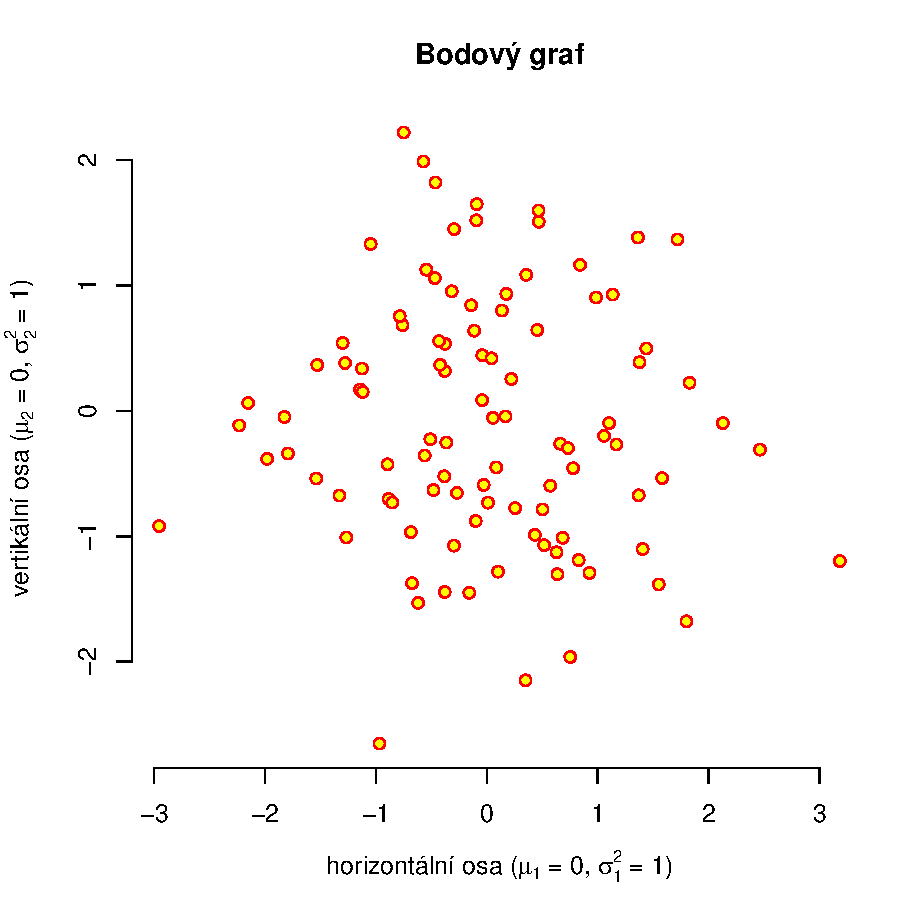
\includegraphics[width=140mm, height=140mm]{../img/ukazka-obr01}
% Příponu není potřeba explicitně uvádět, pdflatex automaticky hledá pdf.
% Rozměry také není nutné uvádět.
\caption{Náhodný výběr z~rozdělení $\mathcal{N}_2(\boldsymbol{0},\,I)$.}
\label{obr03:Nvyber}

\end{figure}

\begin{figure}[p]\centering
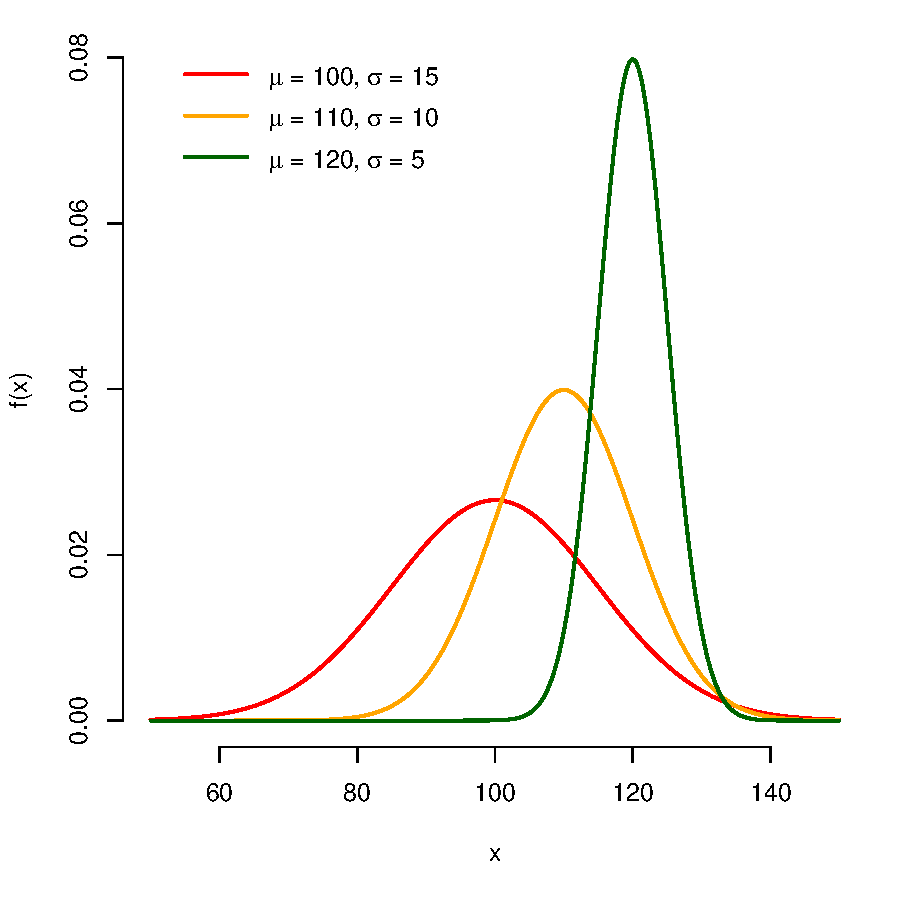
\includegraphics[width=140mm, height=140mm]{../img/ukazka-obr02}
\caption{Hustoty několika normálních rozdělení.}
\label{obr03:Nhust}
\end{figure}

\begin{figure}[p]\centering
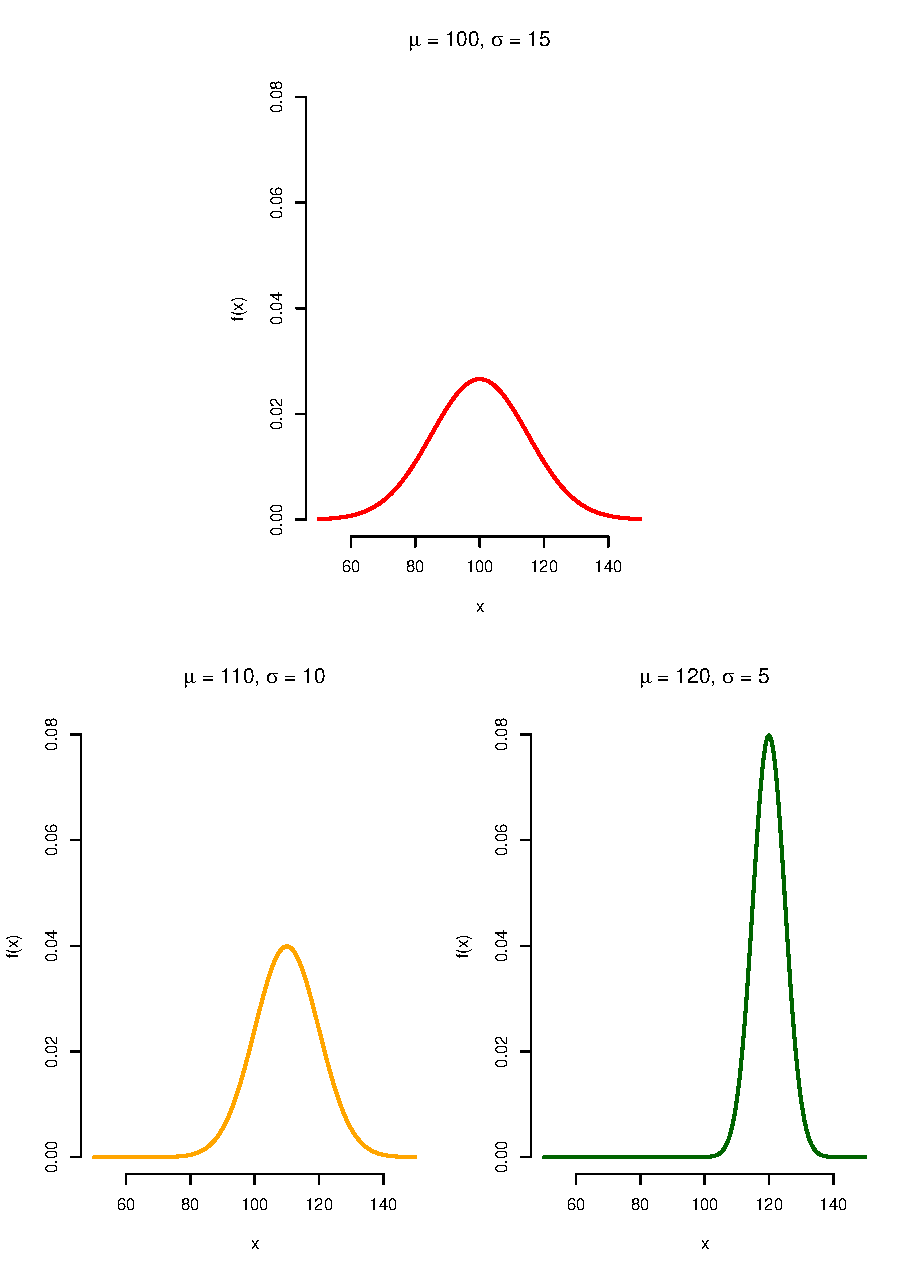
\includegraphics[width=140mm, height=198mm]{../img/ukazka-obr03}
\caption{Hustoty několika normálních rozdělení.}
\label{obr03:Nhust:podruhe}

\end{figure}


\chapter*{Závěr}
\addcontentsline{toc}{chapter}{Závěr}


%%% Seznam použité literatury
%%% Seznam použité literatury je zpracován podle platných standardů. Povinnou citační
%%% normou pro bakalářskou práci je ISO 690. Jména časopisů lze uvádět zkráceně, ale jen
%%% v kodifikované podobě. Všechny použité zdroje a prameny musí být řádně citovány.

\def\bibname{Seznam použité literatury}
\begin{thebibliography}{99}
\addcontentsline{toc}{chapter}{\bibname}

%\bibitem{lamport94}
%  {\sc Lamport,} Leslie.
%  \emph{\LaTeX: A Document Preparation System}.
%  2. vydání.
%  Massachusetts: Addison Wesley, 1994.
%  ISBN 0-201-52983-1.

\end{thebibliography}


%%% Obrázky v bakalářské práci
%%% (pokud jich je malé množství, obvykle není třeba seznam uvádět)
\listoffigures

%%% Tabulky v bakalářské práci (opět nemusí být nutné uvádět)
%%% U matematických prací může být lepší přemístit seznam tabulek na začátek práce.
\listoftables

%%% Použité zkratky v bakalářské práci (opět nemusí být nutné uvádět)
%%% U matematických prací může být lepší přemístit seznam zkratek na začátek práce.
\chapwithtoc{Seznam použitých zkratek}

%%% Přílohy k bakalářské práci, existují-li. Každá příloha musí být alespoň jednou
%%% odkazována z vlastního textu práce. Přílohy se číslují.
%%%
%%% Do tištěné verze se spíše hodí přílohy, které lze číst a prohlížet (dodatečné
%%% tabulky a grafy, různé textové doplňky, ukázky výstupů z počítačových programů,
%%% apod.). Do elektronické verze se hodí přílohy, které budou spíše používány
%%% v elektronické podobě než čteny (zdrojové kódy programů, datové soubory,
%%% interaktivní grafy apod.). Elektronické přílohy se nahrávají do SISu a lze
%%% je také do práce vložit na CD/DVD.
\chapwithtoc{Přílohy}

\openright
\end{document}
